\chapter[Chapter 4]{Solution Design}
\label{sec:chapter4}

\section{Privacy Policy Modeling Language}

StreamGen uses its own language in order to develop DIAs. In this document, StreamGen language is expanded in order to allow users to protect the streams with privacy policies. This expansion consists of a new data stream stereotype in order to specify which streams are protected and with which privacy policy type (VCP or DSEP). Moreover, the sources that generate the Static Context Variables (SCV) and the privacy rules written by the users are also added to the StreamGen language. SCVs are possibly supplied by different sources whilst privacy policies are supposed to be supplied only by one data source type. This sources are inserted in a package which represents the external sources of the DIA following the already existing approach of the StreamGen data types.

Thus, when a stream is protected, the PrivacyProtectingStream stereotype is added to the stream and some properties are filled in order to configure the type of protection. However, defining how the streams must be protected is not enough. Privacy policies require some external data, SCVs and privacy rules, in order to be applied. This two external data are introduced into the DIA by means of two sources, SCV source and privacy rules source. Regarding to the SCVs sources, four different types can be found in this approach. All these types are specified following the already existing approaches of data sources in StreamGen. On the other hand, for the privacy rules source, only one type is defined because the privacy rules file is supposed to be always the same. This two different sources, SCVs source and privacy rules source, are introduced in the application inside of a package stereotype called PrivacyPolicyPackage in order to make more intuitive the approach to the DIA developers.

\subsection{PrivacyProtectingStream}

StreamGen represents the flows of data flowing in DIAs by means of the UML metaclass Information Flow. These flows are known as streams and StreamGen allows to generate some different types as Keyed Stream or Windowed Stream. Each of these types have different characteristics and allow users to generate different behaviors. Moreover, these different streams can be applied all together generating a stream which can be, as in this case, windowed and keyed.

Following this approach, a new stereotype is added to the UML profile of StreamGen. This stereotype is called PrivacyProtectingStream and it is a generalization of the DataStream stereotype, which in turn is an extension of the InformationFlow metaclass. In the figure \ref{fig:PrivacyProtectingStream UML Profile}, the UML profile for the PrivacyProtectingStream is shown.

\begin{figure}
\centering
{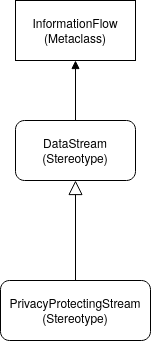
\includegraphics[scale=0.5]{./chapter4/umlProfile/PrivacyProtectingStreamUMLProfile.png}}
\caption{PrivacyProtectingStream UML Profile}
\label{fig:PrivacyProtectingStream UML Profile}
\end{figure}

Regarding to the e-commerce company example explained in the chapter \ref{sec:chapter3}, lets imagine that a user defines a VCP and a DSEP in the same way that they were explained above for such example. The DIA developer, in the profile field of the property window, must specify the PrivacyProtectingStream as an applied stereotypes of the streams S2 and S3, in addition to the required stereotypes (window, keyed, etc.) for these streams. 

Furthermore, PrivacyProtectingStream stereotype have some properties in addition to the already existing property of the DataStream stereotype, isObservable. These properties are:

\begin{itemize}
\item ProtectedByVCP.
\item ProtectedByDSEP.
\item ProtectedStreamConf.
\end{itemize}

ProtectedByVCP and protectedByDSEP properties are added in order to specify how the data stream is protected; if it is protected with a DSEP, with a VCP or if it is protected with both privacy policy types. This is why these two properties are boolean values. Moreover, the configuration of the generated protected stream, which is a stream class imported from the privacy library developed in \cite{privacypoliciesarticle}, has to be specified. In order to define such configuration, a new data type has been added to the UML profile. This data type is called ProtectedStreamConfiguration and it is composed of seven properties. In the tables \ref{PrivacyProtectingStream Properties} and \ref{ProtectedStreamConfiguration Data Type} can be seen a summary of the properties of the PrivacyProtectingStream and the properties of the ProtectedStreamConfiguration data type.

\begin{table}[h!]
\centering
	\begin{tabular}{||c|c|c||} 
	\hline\hline
	Property Name & Property Type & Multiplicity \\ [1ex] 
	\hline\hline
	protectedByVCP & Boolean & 1 \\
	\hline
	protectedByDSEP & Boolean & 1 \\
	\hline
	protectedStreamConf & ProtectedStreamConfiguration & 1 \\
	\hline\hline
	\end{tabular}
\caption{PrivacyProtectingStream Properties}
\label{PrivacyProtectingStream Properties}
\end{table}

\begin{table}[h!]
\centering
	\begin{tabular}{||c|c|c||} 
	\hline\hline
	Property Name & Property Type & Multiplicity \\ [1ex] 
	\hline\hline
	monitoringActive & Boolean & 1 \\
	\hline
	timestampServerIp & String & 1 \\
	\hline
	timeStampServerPort & Integer & 1 \\
	\hline
	topologyParallelism & Integer & 1 \\
	\hline
	simulateRealisticScenario & Boolean & 1 \\
	\hline
	allowedLateness & Integer & 1 \\
	\hline
	logDir & String & 1 \\
	\hline\hline
	\end{tabular}
\caption{ProtectedStreamConfiguration Data Type}
\label{ProtectedStreamConfiguration Data Type}
\end{table}

Regarding to the e-commerce example again, for the stream S2 the protectedByVCP property would be specified as true and for the stream S3 the protectedByDSEP property would be specify to true. Moreover, the values of the ProtectedStreamConfiguration data type would be specified according to the wanted protected stream that the user wants to generate.

The PrivacyProtectingStream allows to easily specify which are the streams that must be protected and with which privacy policy types. This approach does not require any knowledge about the privacy policy types. Moreover, the ProtectedStreamConfiguration can be filled always with the same values, then with an example using such configuration, all the other DIAs could be defined with the same values. The unique value that can vary is the logDir property which is a path and it is not difficult to define a path by a DIA developer. Finally, this approach allows to define the non-privacy-aware dataflow application and, from that application, to add the corresponding privacy configurations over the streams. However, there is no way to specify the SCVs and from where the privacy rules must be read. In order to specify such sources, the PrivacyPolicyPackage is developed.

\subsection{PrivacyPolicyPackage}

StreamGen uses a package stereotype called StreamDatatypes in order to collect all the data types that are flowing through the streams. The data types that are specified inside the package allow users to specify the different values that are conveyed in a stream but inside the same tuple. Following this approach, a new package called PrivacyPolicyPackage is added to the UML profile in order to collect all the privacy sources involved in the privacy-aware dataflow applications, SCV sources and privacy rules source.

These sources are not directly connected to the streams or to the transformations of the DIA but they allow users to specify from where the different external variables required to protect the streams are taken. As they are not directly connected to any operator of the DIA, a package to put all of them together is added to the StreamGen language in order to make the approach more intuitive for the dataflow application developers.

In the figure \ref{fig:PrivacyPolicyPackage UML Profile} can be seen the UML profile of this package. In this image can be seen how the already existing Package metaclass is extended with a stereotype called PrivacyPolicyPackage which goal is to make more intuitive for the DIA developer how to introduce the SCV source and the privacy rules source.

\begin{figure}
\centering
{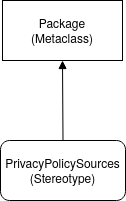
\includegraphics[scale=0.5]{./chapter4/umlProfile/PrivacyPolicyPackageUMLProfile.png}}
\caption{PrivacyPolicyPackage UML Profile}
\label{fig:PrivacyPolicyPackage UML Profile}
\end{figure}

Moreover, in the figure \ref{fig:PrivacyPolicyDataSources Classes UML Profile} can be seen the language of the PrivacyContextSource and PrivacyPolicySource represented in a UML profile diagram. In this figure can be seen how the already existing DataSource stereotype is extended by means of two stereotypes, PrivacyContextSource and PrivacyPolicySource. Moreover, each of these stereotypes are extended as well. As it is explained later, the PrivacyContextSource stereotype is extended by four stereotypes (PrivContTextFileSource, PrivContSocketSource, PrivContKafkaSource, PrivContFixedSource) because the SCV source can be represented by four different type of sources. On the other hand, the PrivacyPolicySource stereotype is extended only by one stereotype (PrivPolYamlFileSource) because it can be represented only by this specific source.

\begin{figure}
\centering
{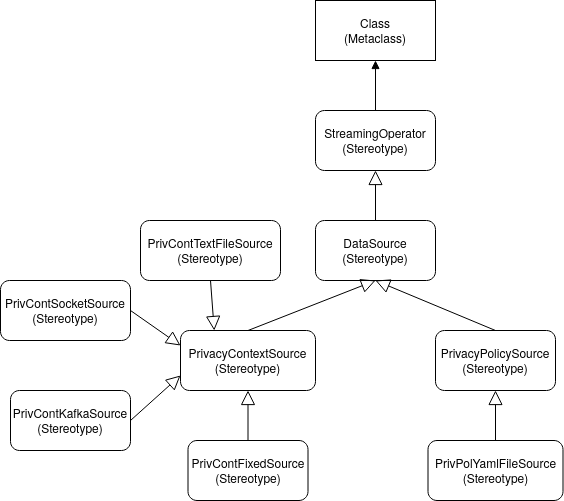
\includegraphics[scale=0.5]{./chapter4/umlProfile/PrivacyPolicyDataSourceUMLProfile.png}}
\caption{PrivacyPolicyDataSources Classes UML Profile}
\label{fig:PrivacyPolicyDataSources Classes UML Profile}
\end{figure}

In order to give an idea about the implementation of this approach, once the PrivacyProtectingStream stereotype is applied on the required streams of the DIA, a package is added to the application model and the PrivacyPolicyPackage stereotype is applied on it in order to make more intuitive to the DIA developer how the external privacy sources would be introduce later.

In summary, independently of the developed DIA, two external sources are always required. A SCV source that specifies the privacy context of the application and a privacy rules source that introduces the privacy policies defined by the users. Moreover, in order to make the approach more intuitive, a package called PrivacyPolicyPackage containing both external sources is added to the StreamGen language.

\subsubsection{PrivacyContextSource}

Static Context Variables (SCVs) are required in order to specify under what conditions privacy policies must be applied. According to \cite{privacypoliciesarticle}, SCVs are always three variables: purpose, role and observer identifier. PrivacyContextSource stereotype provides who is observing the results of the dataflow application. Then, these SCVs can be just a tuple with the three context variables or many tuples with the three variables. This is why a wide variety of possibilities have been developed in order to allow the users to choose the most appropriate SCV source depending on the DIA that is developed. Such possibilities are:

\begin{itemize}
\item PrivContTextFileSource.
\item PrivContSocketSource.
\item PrivContKafkaSource.
\item PrivContFixedSource.
\end{itemize}

Following the approach of StreamGen with data sources, a stereotype called PrivacyContextSource has been created as a generalization of the already existing DataSource stereotype. This new stereotype has four generalizations, the four possibilities among which the user can choose which is the best source for the observer depending on the application. Each of these four sources have its own properties. These properties have been defined taking into account the already existing data sources:

\begin{itemize}
\item TextFileSource.
\item SocketSource.
\item KafkaSource.
\end{itemize}

TextFileSource stereotype reads a file which contains all the input values of the DIA. When the user selects this stereotype the path, (pathToFile) from where the DIA must read the file, is specified. PrivContTextFileSource works exactly in the same way, this stereotype contains a property called pathToFile (String) where the user specifies the path where the file with all the SCV tuples is located. SocketSource stereotype is connected to a port and to a host by means of the properties host (String) and port (Integer) that the user specifies when the stereotype is defined. Following this approach, PrivContSocketSource is connected by a port (Integer) and a host (String) to a server which supplies the SCV tuples.Finally, the KafkaSource is connected by means of kafkaBrokerIp (String) and kafkaBrokerPort (Integer) to a Kafka server. PrivContKafkaSource connects a DIA to a Kafka server that provides the SCV tuples by means of two properties as in the case of the KafkaSource.

In case of PrivContTextFileSource and PrivContSocketSource, when the code is generated a NonParallelStream called contextString which contains the SCV tuples (Strings) is introduced into the DIA. This stream is automatically sent to a map transformation which is imported from the library avoiding that the DIA developer writes any Flink code. This map transformation parses contextString stream to a stream composed with the data type specified by the user in the corresponding package. This data type should contain the same data that each of the strings but the values are split by the comma in order to have each of the values independently. Moreover, this stream is called contextStream and it will be used to apply the privacy policies.

Finally, PrivContFixedSource is a source imported from the library which allows the users to specify only one SCV source. In order to do this, when the user is defining the UML model of the DIA, three properties must be specified. This three properties are fixedUser (String), fixedRole (String) and fixesPuporse (String) which allow to specify the static or fixed SCV source.

In case of PrivContKafkaSource and PrivContFixedSource the contextStream stream with the user specified data type is directly generated without applying any transformation.

In the tables \ref{Privacy Context Source Properties Abstract} can be seen an abstract with all the privacy context sources possibilities, their properties and the multiplicity of each of the properties.

\begin{table}[h!]
\centering
	\begin{tabular}{||c|c|c|c||} 
	\hline\hline
	Privacy Context Source & Property Name & Property Type & Property Multiplicity \\ [1ex] 
	\hline\hline
	PrivContTextFileSource & pathToFile & String & 1 \\
	\hline
	PrivContSocketSource & host & String & 1 \\
	& port & Integer & 1 \\
	\hline
	PrivContKafkaSource & kafkaBrokerIp & String & 1 \\
	& kafkaBrokerPort & Integer & 1 \\
	\hline
	PrivContFixedSource & fixedUser & String & 1 \\
	& fixedRole & String & 1 \\
	& fixesPuporse & String & 1 \\
	\hline\hline
	\end{tabular}
\caption{Privacy Context Source Properties Abstract}
\label{Privacy Context Source Properties Abstract}
\end{table}

In order to apply this privacy approach, after defining the PrivacyPolicyPackage stereotype in the corresponding package node. A class node is introduced in such package and one of the four generalization stereotypes of the PrivacyContextSource stereotype is applied on it. Such stereotype represents the observer of the DIA, in the example of the chapter \ref{sec:chapter3} this sources represents by means of a tuple the employees of a market consultancy.

\subsubsection{PrivacyPolicySource}

In addition to SCVs, StreamGen requires some user specified rules to guarantee privacy. Such privacy rules can be only some simple conditions that have to be satisfied over the stream where the privacy policy is applied or, also, some past conditions satisfied in any stream of the application, both the stream where the privacy policy is applied and any other stream of the application. These rules are supposed to be written in a YAML file that must be inputed to the DIA in order to feed the privacy library Flink codes. In order to handle the YAML file, the library snakeyaml (org.yaml.snakeyaml.Yaml) is used. This is the unique type of sources for such purpose as the rules are supposed to be specified by the user and then stored in a YAML file.

Following the approach of DataSource stereotype, a new stereotype called PrivacyPolicySource is created as a generalization of the DataSource stereotype (figure \ref{fig:PrivacyPolicyDataSources Classes UML Profile}). The goal with this stereotype is to have the possibility to add different type of sources as currently is happening with the SCV source in spite of the approach developed in this document only considers one of them. Moreover, this stereotype makes the language more understandable. From the PrivacyPolicySource stereotype, a new generalization is created in order to make the relationship with a new stereotype called PrivPolYamlFileSource. This stereotype represents the insertion of the YAML file with all the privacy policies specified by the users whose data is handled to the DIA. In order to specify the path where the YAML file is located, a new property (pathToFile, String) is added to the stereotype. With this property, the user is able to define the location where the file is stored and from where the DIA must read the privacy policy rules written by the user. In the table \ref{Privacy Policy Source Property Abstract} can be seen an abstract of such stereotype.

\begin{table}[h!]
\centering
	\begin{tabular}{||c|c|c|c||} 
	\hline\hline
	Privacy Context Source & Property Name & Property Type & Property Multiplicity \\ [1ex] 
	\hline\hline
	PrivPolYamlFileSource & pathToFile & String & 1 \\
	\hline\hline
	\end{tabular}
\caption{Privacy Policy Source Property Abstract}
\label{Privacy Policy Source Property Abstract}
\end{table}

This stereotype follows the example of the TextFileSource stereotype as happened with the PrivContTextFileSource stereotype. However, it is supposed to introduce a YAML file instead of a text file to the dataflow application.

Following how this approach would be applied, after applying the corresponding PrivacyContextSource stereotype in its class, a new class would be introduced in the package with the applied PrivacyPolicyPackage stereotype and the PrivPolYamlFileSource would be applied on it. This source represents the set of privacy rules that the users define, in the example of the chapter \ref{sec:chapter3} the client of the e-commerce company, and that must be applied on the corresponding protected streams.

\section{Privacy Policy Code Generation}

StreamGen exploits Acceleo in order to compile StreamGen language into Spark or Flink languages, depending on the target platform of the dataflow application. In this document, Acceleo is used in order to compile the StreamGen language explained above only into Flink code. Moreover, the developed privacy policy language must be translated in a general way allowing that, independently of the DIA, Flink code must not be modified by the application developer.

The above UML metamodel that specifies the language for the privacy policies must be used by the user in order to create the UML class diagram of the DIA in Papyrus. After that, this diagram is used by Acceleo in order to generate the final code which runs in Flink. In this section all the developed Acceleo codes are explained. Furthermore, all along this section an assumption is taken. This assumption is that the UML file generated by Papyrus is going to contain all the packaged classes in the following order:

\begin{enumerate}
\item Sources.
\item Transformations.
\item Sinks.
\end{enumerate}

First of all, all the sources introducing data are packaged as elements in the UML file that is generated by Papyrus. After them, all the transformations are packaged. Finally, all the sinks where the data must be stored are packaged. This assumption is similar to say that the non-privacy-aware DIA is built in the above order and without adding transformations, sinks or sources after generating the codes of the non-privacy-aware DIA. This is important because due to the approach used for the compilation of the StreamGen language, if this order is not followed, some errors appear when the code is generated. This assumption is taken in the non-privacy-aware StreamGen version too.

In addition to this assumption, the target code generated by means of StreamGen follows a structure that generates the same pieces of code from the UML language specified before.

\subsection{Privacy Policy Codes Structure}

The generated codes for the designed privacy-aware DIA follow a predefined structure in order to use correctly the privacy policy libraries used in \cite{privacypoliciesarticle}. Each of these parts correspond to a different piece of code that is generated taken into account different conditions. Moreover, as specified before, these pieces of code allow to generate the same Flink codes only with slightly modification taken into account the streams of the dataflow application allowing that the approach can be used independetly of the designed DIA. This structure is defined by four parts:

\begin{enumerate}
\item Library Import.
\item Privacy Policy Initialization.
\item Streams Declaration.
\item Streams Protection.
\end{enumerate}

In the Library Import part all the required libraries for the correct code generation operation are called in the corresponding file. Secondly, in the Privacy Policy Initialization part, all the Flink codes for the privacy sources (SCV source and privacy rules source) are generated. After that, in the third part Streams Declaration, all the streams that are not protected are declared in the YAML file in order to follow the approach of \cite{privacypoliciesarticle}. Finally, the streams that must be protected are protected with the privacy library.

\subsubsection{Library Import}

First of all, a condition is required in order to import the libraries of \cite{privacypoliciesarticle} only when they are required. Then, libraries are imported when in the application model exists at least one PrivacyProtectingStream stereotype. If the DIA is non-privacy-aware, there is no PrivacyProtectingStream stereotype and the different libraries are not imported. Such libraries are imported in the file where they are going to be used (generateFlinkApplication.mtl) and the generated piece of code is the following:

\lstinputlisting{./chapters/filesAppen/importedLibraries}

As it can be seen, the imported libraries are:

\begin{itemize}
\item import org.apache.commons.io.FileUtils;
\item import java.io.File;
\item import org.yaml.snakeyaml.Yaml;
\item import it.deib.polimi.diaprivacy.library.GeneralizationFunction;
\item import it.deib.polimi.diaprivacy.library.ProtectedStream;
\item import it.deib.polimi.diaprivacy.model.ApplicationDataStream;
\item import it.deib.polimi.diaprivacy.model.ApplicationPrivacy;
\item import it.deib.polimi.diaprivacy.model.DSEP;
\item import it.deib.polimi.diaprivacy.model.PrivacyContext;
\item import it.deib.polimi.diaprivacy.library.PrivacyContextParser;
\item import it.deib.polimi.diaprivacy.model.VCP;
\item import it.deib.polimi.diaprivacy.library.PrivacyContextFixedSource;
\end{itemize}

The library it.deib.polimi.diaprivacy.library can be found in the repository \url{https://github.com/MicheleGuerriero/dataflow-privacy-library/tree/master/src/main/java/it/deib/polimi/diaprivacy/library}.

Regarding to the library it.deib.polimi.diaprivacy.model, it can be found in the repository \url{https://github.com/MicheleGuerriero/common/tree/master/src/main/java/it/deib/polimi/diaprivacy/model}.

Finally, the org.yaml.snakeyaml.Yaml library must be imported from the POM file. In order to do this, in the POM file generation Acceleo file (generateFlinkPom.mtl), a dependency is triggled when a PrivacyProtectingStream exists in the application model.In the figure \ref{fig:Yaml Dependency POM File} can be seen such generated piece of code.

This is the generated piece of code for such purpose:

\lstinputlisting{./chapters/filesAppen/pomModified}

\subsubsection{Privacy Policy Initialization}

At this part, StreamGen extracts the information supplied by the user in the PrivacyPolicyPackage stereotype. StreamGen generates the corresponding SCV source Flink code and the privacy rules source Flink code. In order to do this, each of the packages contained in the application model are taken and if the package is the PrivacyPolicyPackage, for each of the classes contained in the package a different action is applied taking into account the class type. In the following Acceleo code can be seen the written generation algorithm for the privacy sources.

\lstinputlisting{./chapters/filesAppen/privSrc}

The class types that can be contained in the PrivacyPolicyPackage are:

\begin{itemize}
\item PrivPolYamlFileSource.
\item PrivContFixedSource.
\item PrivContKafkaSource.
\item PrivContTextFileSource.
\item PrivContSocketSource.
\end{itemize}

In the table \ref{Applied Actions for Class Stereotypes in PrivacyPolicySources Package} can be seen an abstract with the actions performed depending on the class type that is included in the PrivacyPolicyPackage. In such table, each of the rows represents: for each class stereotype that can be contained in the PrivacyPolicySources package, the action that is applied.

\begin{table}[h!]
\centering
	\begin{tabular}{||c|c||} 
	\hline\hline
	Class Stereotype & Applied Action \\ [1ex] 
	\hline\hline
	PrivPolYamlFileSource & generateFlinkPrivacyPolicyYamlFileSource  \\
	\hline
	PrivContFixedSource & generateFlinkPrivacyContextFixedSource  \\
	\hline
	PrivContKafkaSource & generateFlinkPrivacyContextKafkaSource  \\
	\hline
	PrivContTextFileSource & generateFlinkPrivacyContextTextFileSource  \\
	\hline
	PrivContSocketSource & generateFlinkPrivacyContextSocketSource  \\
	\hline\hline
	\end{tabular}
\caption{Applied Actions for Class Stereotypes in PrivacyPolicySources Package}
\label{Applied Actions for Class Stereotypes in PrivacyPolicySources Package}
\end{table}

All the actions are applied when there is any of the class stereotypes specified in the table \ref{Applied Actions for Class Stereotypes in PrivacyPolicySources Package} are written in the generateFlinkSources.mtl file of the StreamGen Acceleo project as public templates.

In the following commented codes can be seen the examples of such generation actions for the class stereotypes PrivPolYamlFileSource and PrivContTextFileSource.

\lstinputlisting{./chapters/filesAppen/privSrcExamples}

\subsubsection{Streams Declaration}

This document works with the already defined YAML file structure in the repository of \cite{privacypoliciesarticle}. This YAML file owns a field called concreteStream that is null when the YAML file is introduced. This field must be filled for all the streams flowing through the application because later the field is used by the library to protect the streams in the Streams Protection part. Then, after generating and parsing the SCVs and the privacy policy YAML file in the Privacy Policy Initialization part, StreamGen declares all those streams that are introduced to a transformation and that the PrivacyProtectingStream stereotype is not applied on them. Regardless of what stream is considered, they are non-protected once in the application. If the application does not protected a stream, the stream exists only without privacy protection. However, if the stream is protected, first of all the non-protected version of the stream is generated and, then, the stream is protected. This is why, every generated stream by a transformation that is not protected, it is declared in the YAML file. In order to do this, a condition must be taken in account every time that a stream is generated by means of a transformation. Such condition is the same condition considered in order to import the libraries; when in the application model exists at least one PrivacyProtectingStream stereotype, then the the output stream of the transformation must be declared in the YAML file. In the following Acceleo code can be seen the piece of code written for such purpose. This piece of code is replicated in all the existing transformations of StreamGen (generateFlinkTransformations.mtl).

\lstinputlisting{./chapters/filesAppen/streamDeclaration}

Thus, any time that a transformation is generated, after generating the piece of code corresponding to the transformation, one conditions is taken into account. This condition checks that exists at least one PrivacyProtectingStream stereotype in the application model. If such condition is satisfied, then, the stream is set into the privacy policy YAML file.

\subsubsection{Streams Protection}

StreamGen consists of three different types of operators: sources, transformations and sinks. Sources introduce some strings that must be parsed by a transformation in order to generate a data type. This happens independently of the implemented data source. Transformations make some computation modifying and generating new data types. Finally, some of the generated data types are stored in a sink.

On the other hand, a transformation can introduce a pair of streams (CoFlatMap and CoMap transformation) and, also, it can generate several streams. StreamGen is implemented in a way that assumes that all the generated streams are the same stream. Then, in spite of several streams must be specified in the UML diagram, Acceleo takes only one of such outputs in order to generate the transformation. Following this approach, privacy policies are going to be generated only once assuming that all the privacy output streams of a transformation are the same stream.

Then, the Acceleo algorithm developed in StreamGen is extended. Before extending the algorithm, StreamGen checks one by one all the transformations that are contained in the application model and depending on the applied stereotype to the classes, generates different actions. If this is not modified, it allows to generate all the streams, regardless of whether they are protected. Once the non-protected stream generated by the transformation is created, an extension of the algorithm is made. A condition is taken into account in order to check if the output stream must be protected or if it must not. In order to do this, if exists an output stream from the transformation that contains the stereotype PrivacyProtectingStream, an action called generateFlinkPrivPolicies is executed. An example for the SocketSource, MapTransformation and TextFileSink stereotypes of the extended algorithm is presented in the figures \ref{fig:Triggering SocketSource Privacy StreamGen Version}, \ref{fig:Triggering MapTransformation Privacy StreamGen Version} and \ref{fig:Triggering TextFileSink Privacy StreamGen Version}. As it can be seen there, the protection over the streams is only applied on the output streams of the transformations. This ensures that any stream is protected only once as it takes only one of all the replicas of the output streams. Moreover, two assumptions are taken. The first one is that any source requires a parser to transform the input stream into a DIA data type. The second one is that all the output streams generated by a transformation are protected with the same privacy policy types (VCP, DSEP or both of them).

\begin{figure}
\centering
{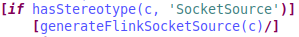
\includegraphics[scale=0.5]{./chapter4/codeStructure/SocketSourcePrivacyVersion.png}}
\caption{Triggering SocketSource Privacy StreamGen Version}
\label{fig:Triggering SocketSource Privacy StreamGen Version}
\end{figure}

\begin{figure}
\centering
{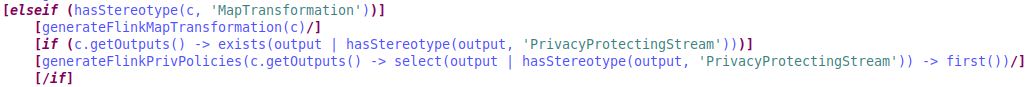
\includegraphics[scale=0.3]{./chapter4/codeStructure/MapTransformationPrivacyVersion.png}}
\caption{Triggering MapTransformation Privacy StreamGen Version}
\label{fig:Triggering MapTransformation Privacy StreamGen Version}
\end{figure}

\begin{figure}
\centering
{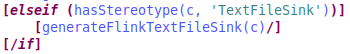
\includegraphics[scale=0.5]{./chapter4/codeStructure/TextFileSinkPrivacyVersion.png}}
\caption{Triggering TextFileSink Privacy StreamGen Version}
\label{fig:Triggering TextFileSink Privacy StreamGen Version}
\end{figure}

This extended algorithm triggers the generateFlinkPrivPolicies action. Such action consists of four steps and it is written in the generateFlinkTransformations.mtl file of the StreamGen project. Moreover, this action takes advantage of the privacy library.

First of all, the stream declared in the Streams Declaration part is called. In the figure \ref{fig:Calling Declared Stream} can be seen how the declared stream is called. After that, a protected stream with the values specified in the ProtectedStreamConfiguration data type of the property protectedStreamConf of the PrivacyProtectingStream stereotype is generated. Then, taking into account if the stream is VCP or DSEP protected with the properties: protectedByVCP and protectedByDSEP, the VCPs and DSEPs of the YAML file are added to the protected stream previously declared. Such step can be seen how is developed in the figure \ref{fig:Adding Privacy Policies}. Finally, all the privacy policies are applied on the stream. This steps takes advantage of the finalize method developed in the privacy library. The step is specified in the figure \ref{fig:Applying Privacy Policies}.

\begin{figure}
\centering
{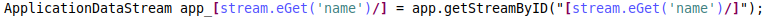
\includegraphics[scale=0.3]{./chapter4/codeStructure/CallingDeclaredStream.png}}
\caption{Calling Declared Stream}
\label{fig:Calling Declared Stream}
\end{figure}

\begin{figure}
\centering
{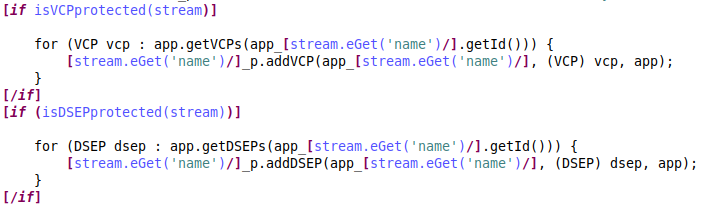
\includegraphics[scale=0.3]{./chapter4/codeStructure/AddingPrivacyPolicies.png}}
\caption{Adding Privacy Policies}
\label{fig:Adding Privacy Policies}
\end{figure}

\begin{figure}
\centering
{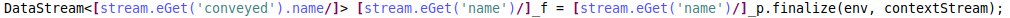
\includegraphics[scale=0.3]{./chapter4/codeStructure/ApplyingPrivacyPolicies.png}}
\caption{Applying Privacy Policies}
\label{fig:Applying Privacy Policies}
\end{figure}



















